\documentclass[12pt]{article}
\usepackage[left=1cm, right=1cm, top=2cm,bottom=1.5cm]{geometry} 

\usepackage[parfill]{parskip}
\usepackage[utf8]{inputenc}
\usepackage[T2A]{fontenc}
\usepackage[russian]{babel}
\usepackage{enumitem}
\usepackage[normalem]{ulem}
\usepackage{amsfonts, amsmath, amsthm, amssymb, mathtools}
\usepackage{tabularx}
\usepackage{hhline}

\usepackage{accents}
\usepackage{fancyhdr}
\pagestyle{fancy}
\renewcommand{\headrulewidth}{1.5pt}
\renewcommand{\footrulewidth}{1pt}

\usepackage{graphicx}
\usepackage[figurename=Рис.]{caption}
\usepackage{subcaption}
\usepackage{float}

%%Наименование папки откуда забирать изображения
\graphicspath{ {./images/} }

%%Изменение формата для ввода доказательства
\renewcommand{\proofname}{$\square$  \nopunct}
\renewcommand\qedsymbol{$\blacksquare$}

%%Изменение отступа на таблицах
\addto\captionsrussian{%
	\renewcommand{\proofname}{$\square$ \nopunct}%
}
%% Римские цифры
\newcommand{\RN}[1]{%
	\textup{\uppercase\expandafter{\romannumeral#1}}%
}

%% Для удобства записи
\newcommand{\MR}{\mathbb{R}}
\newcommand{\MC}{\mathbb{C}}
\newcommand{\MQ}{\mathbb{Q}}
\newcommand{\MN}{\mathbb{N}}
\newcommand{\MTB}{\mathbb{T}}
\newcommand{\MTI}{\mathbb{I}}
\newcommand{\MI}{\mathrm{I}}
\newcommand{\MJ}{\mathrm{J}}
\newcommand{\MH}{\mathrm{H}}
\newcommand{\MT}{\mathrm{T}}
\newcommand{\MU}{\mathcal{U}}
\newcommand{\MV}{\mathcal{V}}
\newcommand{\MB}{\mathcal{B}}
\newcommand{\MW}{\mathcal{W}}
\newcommand{\ML}{\mathcal{L}}
\newcommand{\VN}{\varnothing}
\newcommand{\VE}{\varepsilon}

\theoremstyle{definition}
\newtheorem{defn}{Опр:}
\newtheorem{rem}{Rm:}
\newtheorem{prop}{Утв.}
\newtheorem{exrc}{Упр.}
\newtheorem{lemma}{Лемма}
\newtheorem{theorem}{Теорема}
\newtheorem{corollary}{Следствие}

\newenvironment{cusdefn}[1]
{\renewcommand\thedefn{#1}\defn}
{\enddefn}

\DeclareRobustCommand{\divby}{%
	\mathrel{\text{\vbox{\baselineskip.65ex\lineskiplimit0pt\hbox{.}\hbox{.}\hbox{.}}}}%
}
%Короткий минус
\DeclareMathSymbol{\SMN}{\mathbin}{AMSa}{"39}
%Длинная шапка
\newcommand{\overbar}[1]{\mkern 1.5mu\overline{\mkern-1.5mu#1\mkern-1.5mu}\mkern 1.5mu}
%Функция знака
\DeclareMathOperator{\sgn}{sgn}

%Функция ранга
\DeclareMathOperator{\rk}{\text{rk}}

%Обозначение константы
\DeclareMathOperator{\const}{\text{const}}

\DeclareMathOperator*{\dsum}{\displaystyle\sum}
\newcommand{\ddsum}[2]{\displaystyle\sum\limits_{#1}^{#2}}

%Интеграл в большом формате
\DeclareMathOperator{\dint}{\displaystyle\int}
\newcommand{\ddint}[2]{\displaystyle\int\limits_{#1}^{#2}}
\newcommand{\ssum}[1]{\displaystyle \sum\limits_{n=1}^{\infty}{#1}_n}

\newcommand{\smallerrel}[1]{\mathrel{\mathpalette\smallerrelaux{#1}}}
\newcommand{\smallerrelaux}[2]{\raisebox{.1ex}{\scalebox{.75}{$#1#2$}}}

\newcommand{\smallin}{\smallerrel{\in}}
\newcommand{\smallnotin}{\smallerrel{\notin}}

\newcommand*{\medcap}{\mathbin{\scalebox{1.25}{\ensuremath{\cap}}}}%
\newcommand*{\medcup}{\mathbin{\scalebox{1.25}{\ensuremath{\cup}}}}%

\makeatletter
\newcommand{\vast}{\bBigg@{3.5}}
\newcommand{\Vast}{\bBigg@{5}}
\makeatother

%Промежуточное значение для sup\inf, поскольку они имеют разную высоту
\newcommand{\newsup}{\mathop{\smash{\mathrm{sup}}}}
\newcommand{\newinf}{\mathop{\mathrm{inf}\vphantom{\mathrm{sup}}}}

%Скалярное произведение
\DeclarePairedDelimiterX{\inner}[2]{\langle}{\rangle}{#1, #2}

%Подпись символов снизу
\newcommand{\ubar}[1]{\underaccent{\bar}{#1}}

%% Шапка для букв сверху
\newcommand{\wte}[1]{\widetilde{#1}}

%%Функция для обозначения равномерной сходимости по множеству
\newcommand{\uconv}[1]{\overset{#1}{\rightrightarrows}}

%%Функция для обозначения нижнего и верхнего интегралов
\def\upint{\mathchoice%
	{\mkern13mu\overline{\vphantom{\intop}\mkern7mu}\mkern-20mu}%
	{\mkern7mu\overline{\vphantom{\intop}\mkern7mu}\mkern-14mu}%
	{\mkern7mu\overline{\vphantom{\intop}\mkern7mu}\mkern-14mu}%
	{\mkern7mu\overline{\vphantom{\intop}\mkern7mu}\mkern-14mu}%
	\int}
\def\lowint{\mkern3mu\underline{\vphantom{\intop}\mkern7mu}\mkern-10mu\int}


\begin{document}
\lhead{Математический анализ - \RN{3}}
\chead{Шапошников С.В.}
\rhead{Лекция - 13}
\section*{Свойства равномерно сходящихся последовательностей}

\subsection*{Теорема Арцела (первое доказательство)}
Мы будем рассматривать множества, которые есть объединения отрезков, но не любых, а которые не более чем счетные и могут пересекаться лишь по концам:
$$
	F = \bigcup\limits_{n} \Delta_n \subset [a,b], \, \Delta_n = [a_n, b_n], \, \forall n \neq m, \, \Delta_n \cap \Delta_m = 
	\begin{cases}
		\VN, \\
		b_n = a_m \vee b_m = a_n,
	\end{cases}
$$
\begin{figure}[H]
	\centering
	\includegraphics[width=0.65\textwidth]{MA3L13_1.eps}
	\label{MA3L13_1}
	\caption{Расположение отрезков $\Delta_n$ и $\Delta_m$, при $n \neq m$.}
	\label{fig:Покрытие	}
\end{figure}
По-другому это можно записать так: $\mathring{\Delta}_n \cap \mathring{\Delta}_m = \VN, \, \forall n \neq m$, где $\mathring{\Delta}$ означет внутренность интервала $\Delta$. Каждому такому множеству $F$ мы можем приписать длину $\lambda(F)$: 
$$
	\lambda(F) = \sum\limits_{n}|\Delta_n|
$$ 
Порядок нумерования отрезков - не важен, поскольку абсолютно сходящийся ряд не меняет своей суммы от перестановки мест слагаемых. Чтобы не разбираться с вопросами, что одно и то же множество можно представить в виде разных объединений $\Delta_n$, мы будем считать, что множество идет всегда в паре с набором отрезков. Далее рассматриваем множества только такого вида. 
\begin{prop}
	Если $F \subset \displaystyle \bigcup\limits_n F_n$, то $\lambda(F) \leq \displaystyle\sum\limits_{n} \lambda(F_n)$.
\end{prop}
\begin{proof}
	По условию:
	$$
		F = \bigcup\limits_{k} \Delta_k \subset \bigcup\limits_n F_n, \, F_n = \bigcup\limits_{j } \Delta_j^n \Rightarrow \forall k, \, \Delta_k \subset \bigcup\limits_{j,n}\Delta_j^n 
	$$
	по лемме $3$, лекции $24$ из прошлого семестра будет верно, что длина отрезка $\Delta_k$ меньше, чем сумма длин покрывающих отрезков, от которых всегда можно оставить кусок, относящийся только к $\Delta_k$:
	$$
		|\Delta_k| \leq \sum\limits_{j,n}\left|\Delta_j^n \cap \Delta_k\right |
	$$
	Поскольку $\mathring{\Delta}_n \cap \mathring{\Delta}_m = \VN, \, \forall n \neq m$, то по лемме $2$ лекции $25$ прошлого семестра:
	$$
		\bigcup\limits_{k = 1}^{M}(\Delta_j^n \cap \Delta_k ) \subset \Delta_j^n \Rightarrow \sum\limits_{k = 1}^M\left|\Delta_j^n \cap \Delta_k\right | \leq |\Delta_j^n| 
	$$
	Тогда рассматривая не более чем счетное объединение множеств:
	$$
		\bigcup\limits_{k = 1}^{\infty}(\Delta_j^n \cap \Delta_k )  \subset \Delta_j^n \Rightarrow \forall M, \, \bigcup\limits_{k = 1}^{M}(\Delta_j^n \cap \Delta_k )  \subset \Delta_j^n \Rightarrow \forall M,\, \sum\limits_{k = 1}^M\left|\Delta_j^n \cap \Delta_k\right | \leq |\Delta_j^n| 
	$$
	Переходя к пределу по $M \to \infty$ мы получим:
	$$
		\sum\limits_{k = 1}^{\infty}\left|\Delta_j^n \cap \Delta_k\right | \leq |\Delta_j^n|
	$$
	или воспользовавшись тем, что частичные суммы знакопостоянного ряда ограничены сверху. Поскольку мы рассматриваем множества вида $F \subset [a,b]$, то:
	$$
		J = \bigcup\limits_{n} F_n \subset [a,b] \Rightarrow \lambda(J) \leq \lambda(J) +  \lambda([a,b]\setminus J) = \lambda([a,b]) = \left|[a,b]\right| = b-a < \infty
	$$
	Тогда, сумма ряда по пересечениям отрезков будет абсолютно сходиться, поскольку:
	$$
		\bigcup\limits_{k}\bigcup\limits_{j,n} (\Delta_j^n \cap \Delta_k) \subset F \subset [a,b] \Rightarrow \sum\limits_{k}\sum\limits_{j,n}\left|\Delta_j^n \cap \Delta_k\right| < b - a < \infty
	$$
	Вспоминая, что при абсолютной сходимости можно писать сумму в любом порядке, мы получим:
	$$
		\lambda(F) = \sum\limits_{k}|\Delta_k| \leq \sum\limits_{k}\sum\limits_{j,n}\left|\Delta_j^n \cap \Delta_k\right| = \sum\limits_{j,n}\sum\limits_{k}\left|\Delta_j^n \cap \Delta_k\right| \leq \sum\limits_{j,n}|\Delta_j^n| = \sum\limits_{n}\lambda(F_n)
	$$
\end{proof}
\begin{rem}
	На самом деле в доказательстве есть тонкий момент, касающийся рядов $\displaystyle \sum\limits_{n,m}|a_{n,m}|$. 
	
	Почему можно переставлять слагаемые и суммировать в любом порядке? Это похоже на теорему о том, что абсолютно сходящийся ряд можно переставлять в любом порядке, но это не совсем она. Мы хотим:
	$$
		\sum\limits_{n,m}|a_{nm}| = \sum\limits_{n}\sum\limits_{m}|a_{nm}|
	$$
	это не тоже самое, что и переставить как угодно. Это сложение по каждой строке, а затем суммирование по тому, что получилось или наоборот. См. Фихтенгольца про повторные ряды или последующие лекции (это будет обсуждаться далее).
\end{rem}
\begin{prop}
	Пусть есть последовательность вложенных множеств: $F_1 \supset F_2 \supset \dotsc \supset F_n \supset \dotsc$. Причем известно, что $\forall n, \, \lambda(F_n) \geq \delta > 0$, тогда пересечение не может быть пустым: $\displaystyle \bigcap\limits_{n} F_n \neq \VN$.
\end{prop}
\begin{rem}
	Смысл утверждения в том, что у вложенных друг в друга множеств длина которых не падает к нулю, поэтому там должно что-то оставаться в пересечении. Если бы выжимались в пустое множество, то там бы и длина падала.
\end{rem}
\begin{proof}
	Возьмем $F_n$, его можно представить в виде объединения отрезков: 
	$$
		\forall n, \, F_n = \displaystyle \bigcup\limits_{j}\Delta_j^n \subset [a,b]
	$$ 
	Мы рассматриваем только такие множества. Заметим, что следующий ряд сходится: 
	$$
		\sum\limits_{j}|\Delta_j^n| \leq b - a < \infty
	$$ 
	Это так, поскольку мы берем отрезки внутри $[a,b]$, которые пересекаются лишь по концам $\Rightarrow$  любая конечная сумма этих отрезков будет оцениваться длиной отрезка $[a,b]$: 
	$$
		\bigcup\limits_{j = 1}^{\infty}\Delta_j^n \subset [a,b] \Rightarrow \forall M, \, \bigcup\limits_{j = 1}^{M}\Delta_j^n   \subset [a,b] \Rightarrow \forall M,\, \sum\limits_{j = 1}^M\left|\Delta_j^n \right| \leq \left|[a,b]\right| = b - a < \infty 
	$$
	Переходя в неравенстве к пределу по $M \to \infty$, мы получим:
	$$
		\bigcup\limits_{j = 1}^{\infty}\Delta_j^n \subset [a,b] \Rightarrow \sum\limits_{j = 1}^{\infty}\left|\Delta_j^n \right| \leq \left|[a,b]\right| = b - a < \infty 	
	$$
	Таким образом, сумма отрезков $\Delta_j^n$ конечна $\Rightarrow$ можно выбрать сколь угодно малый хвост:
	$$
		\forall \delta > 0, \, \forall n, \, \exists \, N_n \colon \bigcup\limits_{j = N_n + 1 }^{\infty}\Delta_j^n \subset \bigcup\limits_{j = 1}^{\infty}\Delta_j^n \colon \sum\limits_{j = N_n + 1}^{\infty}|\Delta_j^n| < \dfrac{\delta}{2^{n+1}}
	$$
	Обозначим через $K_n$ объединение первых $N_n$ отрезков:
	$$
		\forall n, \, K_n = \bigcup\limits_{j = 1}^{N_n}\Delta_j^n
	$$
	очевидно, что такие множества - компакты (конечное объединение отрезков). Тогда:
	$$
		\forall n, \, F_n \setminus K_n \subset \wte{F_n \setminus K_n}  = \bigcup\limits_{j = N_n + 1}^{\infty}\Delta_j^n \Rightarrow \wte{F_n \setminus K_n} = \left(F_n \setminus K_n \right) \cup \{c \colon c \in \MI\}
	$$
	где $\MI_n$ - множество концов отрезков, выброшенных при вычете множества $K_n$ из $F_n$. Тогда очевидно:
	$$
		\lambda\left(\wte{F_n \setminus K_n}\right) = \sum\limits_{j = N_n + 1}^{\infty}|\Delta_j^n| < \dfrac{\delta}{2^{n+1}}
	$$
	Пересечем эти компакты $K_n$ следующим образом:
	$$
		\forall M, \, K^M = \bigcap\limits_{n = 1}^M K_n = \bigcap\limits_{n = 1}^M \left(\bigcup\limits_{j = 1}^{N_n} \Delta_j^n \right) 
	$$
	Полученное множество также будет являться компактом, поскольку пересечение компактов это их замкнутое подмножество $\Rightarrow$ это компакт. Предположим, что пересечение $K^M$ не пусто, тогда:
	$$
		\bigcap\limits_{M = 1}^{\infty} K^M \neq \VN \Rightarrow \bigcap\limits_{n = 1}^{\infty} K_n \neq \VN
		\Rightarrow \bigcap\limits_{n = 1}^{\infty} F_n \neq \VN
	$$
	поскольку, если в пересечении $K_n$ что-то есть, то это же будет и в пересечении $F_n$. Пусть пересечение по $K^M$ будет пусто, тогда:
	$$
		\bigcap\limits_{M = 1}^{\infty} K^M = \VN \Rightarrow \exists \, T \colon K^{T} = \VN
	$$
	Это так, поскольку мы получили вложенную систему компактов:
	$$
		\forall M, \, K^M = \bigcap\limits_{n = 1}^M K_n \Rightarrow K^1 \supset K^2 \supset \dotsc K^M \supset K^{M+1} \supset \dotsc
	$$
	если каждый из них не пуст, то в каждом можно взять точку $\Rightarrow$ это будет подмножество точек компакта, например, $K^1 \Rightarrow$ из последовательности точек компакта выберем сходящуюся подпоследовательность: 
	$$
		\forall M, \, K^M \neq \VN \Rightarrow  \forall M, \, \exists \, x_M \colon x_M \in K^M \Rightarrow \{x_M\} \in K^1 \Rightarrow \exists\, x_{M_j} \in \{x_M\} \colon x_{M_j} \to x_0 \in K^1
	$$	
	Поскольку $K^M$ - вложенные, то начиная с некоторого номера, все члены этой подпоследовательности будут лежать в каждом из указанных компактов $\Rightarrow$ в силу замкнутости компакта, предел также будет лежать в каждом $K^M$ (предел в замкнутом множестве принадлежит этому же множеству):
	$$
		\forall M, \, \exists \, N \colon \forall j > N, \, x_{M_j} \in K^M \Rightarrow x_0 \in K^M
	$$
	Возьмем $K^{T}$, поскольку оно пустое, то его можно выбрасывать откуда угодно:
	$$
		F_T = F_T \setminus K^{T} = F_T \setminus \left(\bigcap\limits_{n = 1}^T K_n\right) = \bigcup\limits_{n = 1}^T \left(F_T \setminus K_n\right)
	$$
	Поскольку по условию $F_1 \supset F_2 \supset \dotsc \supset F_n \supset \dotsc$, то мы перепишем равенство выше так:
	$$
		F_T = \bigcup\limits_{n = 1}^T \left(F_T \setminus K_n\right) \subset \bigcup\limits_{n = 1}^T \left(F_n \setminus K_n\right) \subset \bigcup\limits_{n = 1}^T \left(\wte{F_n \setminus K_n}\right)
	$$
	По утверждению $1$ мы получим следующее:
	$$
		\delta \leq \lambda(F_T) \leq \sum\limits_{n = 1}^T \lambda\left(\wte{F_n \setminus K_n}\right) < \sum\limits_{n = 1}^T \dfrac{\delta}{2^{n+1}} < \sum\limits_{n = 1}^{\infty} \dfrac{\delta}{2^{n+1}} = \dfrac{\delta}{2}
	$$
	Получили противоречие $\Rightarrow$ невозможно, что пересечение $K^M$ - пусто.
\end{proof}
\begin{rem}
	Заметим, что $F_n$ содержат счетное число отрезков, они не обязательно компакты. Если бы они были компактами, то зная что они все не пусты, мы бы знали, что у них непустое пересечение. Поэтому идея состоит в том, чтобы заменить $F_n$ компактами, но делая такую замену, надо убедиться что в какой-то моент эти компакты не станут пустыми. Для этого надо выбирать компакты, которые тоже будут иметь достаточно большую длину. Тогда если компакт схлопнется, то он просто изничтожит соответствующие $F_n$.
\end{rem}
Докажем также вспомогательное утверждение для доказательства теоремы.
\begin{prop}
	Если $f_n$ - интегрируемы на $[a,b]$ по Риману, $C \geq f_n \geq 0, \, f_n(x) \to 0$ сходятся поточечно к нулю и $\forall n, \, \exists \, \MTB_n$ - разбиение отрезка $[a,b]$ такое, что $\forall n , \, \MTB_n \subset \MTB_{n+1}$. Тогда:
	$$
		\forall \VE > 0, \, \forall \delta > 0, \, \exists \, N \colon \forall n > N, \, \MI = \left\{j \colon \inf\limits_{\Delta_j^n}f_n \geq \VE\right\}, \, \sum\limits_{j \in \MI} |\Delta_j^n| \leq \delta
	$$
\end{prop}
\begin{proof}

	\begin{figure}[H]
		\centering
		\includegraphics[width=0.55\textwidth]{MA3L13_2.png}
		\label{MA3L13_2}
		\caption{Сумма длин отрезков на интервалах, где $\inf\limits_{\Delta_j^n}f_n \geq \VE$ меньше $\delta$.}
		\label{fig:Сумма длин отрезков}
	\end{figure}
	Предположим противное. Нечто неверно, начиная с некоторого номера, означает, что $\exists$ бесконечная последовательность номеров для которой это нечто будет неверно $\Rightarrow$ существует возрастающая последовательность номеров $\{n_j\}$ такая, что сумма длин отрезков, где точная нижняя грань $f_{n_j}$ больше $\VE$ будет больше, чем $\delta$:
	$$
		\exists \, \{n_j\} \colon \sum\limits_{k \in \MI}|\Delta_k^{n_j}| > \delta, \, \MI = \left\{k \colon \inf\limits_{\Delta_k^{n_j}}f_{n_j} \geq \VE\right\}
	$$
	Составим из полученных отрезков множества:
	$$
		F_m = \bigcup\limits_{j \geq m}\left\{ \Delta_k^{n_j} \colon \inf\limits_{\Delta_k^{n_j}}f_{n_j}\geq \VE \wedge \forall r,t, \, \forall s \neq q, \, \mathring{\Delta}_t^{n_s} \cap \mathring{\Delta}_r^{n_q} = \VN \right\}
	$$
	то есть, мы отходим достаточно далеко по номерам $j$, начиная с номера $m$ и скидываем в кучу ``плохие'' отрезки. Поскольку разбиения вложенные: $\MTB_{n_j} \subset \MTB_{n_{j+1}}$, то каждый раз отрезки, которые появляются на следующем шаге либо содержатся внутри уже имеющихся, либо добавляются к ним:
	$$
		j = m \Rightarrow \Delta_{k_1}^{n_m}, \dotsc, \Delta_{k_{l_m}}^{n_m} \in \MTB_{n_m}	\colon \forall i = \overline{1, l_m}, \, \inf\limits_{\Delta_{k_i}^{n_m}}f_{n_m}\geq \VE
	$$
	$$
		j = m + 1 \Rightarrow \Delta_{k_1}^{n_{m+1}}, \dotsc, \Delta_{k_{l_{m+1}}}^{n_{m+1}} \in \MTB_{n_{m+1}}	\colon \forall i = \overline{1, l_{m+1}}, \, \inf\limits_{\Delta_{k_i}^{n_{m+1}}}f_{n_{m+1}}\geq \VE
	$$
	\begin{figure}[H]
		\centering
		\includegraphics[width=0.55\textwidth]{MA3L13_4.png}
		\label{MA3L13_4}
		\caption{Добавление новых отрезков в $F_m$: зеленые - добавляются, красные - уже были включены ранее.}
		\label{fig:Добавление новых отрезков}
	\end{figure}
	Вычеркиваем те отрезки, которые лежат уже внутри учтенных отрезках, опять же это возможно из-за вложенности разбиения. Продолжаем это для всех $j > m + 1$. 
	
	Таким образом, $F_m$ имеет ровно тот вид, который мы представляли ранее - объединение попарно непересекающихся по внутренностям отрезков. Очевидно, что $\lambda(F_m) > \delta$, поскольку:
	$$
		\bigcup\limits_{i = 1}^{l_m}\Delta_{k_i}^{n_m}\subset F_m \Rightarrow \lambda(F_m) \geq \lambda\left(\bigcup\limits_{i = 1}^{l_m}\Delta_{k_i}^{n_m}\right) = \left|\Delta_{k_1}^{n_m}\right| +  \dotsc + \left|\Delta_{k_{l_m}}^{n_m}\right| > \delta
	$$
	Одновременно с этим, по построению верно $F_1 \supset F_2 \supset \dotsc F_m \supset F_{m+1} \supset \dotsc$, потому что каждый раз начинаем со следующего более высокого номера, а значит в предыдущих оно точно содержалось. Тогда по утверждению $2$ пересечение всех $F_m$ не пусто.
	
	Пусть $x_0 \in \bigcap\limits_{m} F_m \neq \VN$, утверждается, что в точке $x_0$ последовательность $f_n(x_0)$ не сходится к нулю: мы брали отрезки со сколь угодно далекими номерами $n_j \Rightarrow$ есть подпоследовательность функций, каждая из которой в этой точке $x_0$ отделена от нуля значением $\VE \Rightarrow$ не сходится к нулю (если сходится, то любая подпоследовательность сходится к тому же пределу, а здесь это не так) $\Rightarrow$ получили противоречие.
\end{proof}

\begin{theorem}(\textbf{Арцела})
	Если $f_n, f$ - интегрируемы на $[a,b]$ по Риману, последовательность - ограничена: $\forall n, x, \, |f_n(x)| \leq C$ (равномерно ограничены) и $f_n(x) \to f(x)$ поточечно, то:
	$$
		\lim\limits_{n \to \infty} \ddint{a}{b}f_n(x) dx = \ddint{a}{b}f(x)dx
	$$
\end{theorem}
\begin{proof}
	Достаточно доказать только в следующем частном случае:
	$$
		C \geq f_n \geq 0, \, f_n \to 0 \Rightarrow \ddint{a}{b}f_n(x)dx \to 0
	$$
	Для понимания этого факта, рассмотрим следующую разность:
	$$
		\left|\ddint{a}{b}f_n(x)dx - \ddint{a}{b}f(x)dx\right| \leq \ddint{a}{b}\left|f_n(x) - f(x)\right|dx \to 0 
	$$
	где верно следующее: $\forall n, \, |f_n(x) - f(x) | \geq 0 \wedge \lim\limits_{n \to \infty}|f_n(x) - f(x)| = 0$. Таким образом, это эквивалентно нашему частному случаю. Рассмотрим его, поскольку все функции $f_n$ - интегрируемы на $[a,b]$, то по критерию Дарбу нижний и верхний интегралы Дарбу равны и равны интегралу по $f_n$:
	$$
		\underline{\MI} = \overline{\MI} = \int\limits_{a}^{b}f_n(x) dx
	$$
	
	По определению нижнего интеграла Дарбу (см. лекцию $24$ прошлого семестра) мы знаем, что: 
	$$
		\ddint{a}{b}f_n(x)dx = \underline{\MI} = \sup\limits_{\MTB}s(f_n,\MTB)
	$$
	поэтому, поскольку нижний интеграл Дарбу это точная верхняя грань нижней суммы Дарбу, то:
	$$
		\forall n, \, \exists \, \MTB_n \text{ - разбиение отрезка} \, [a,b] \colon \ddint{a}{b} f_n(x)dx - s(f_n, \MTB_n) < \dfrac{1}{n}
	$$
	Более того, по лемме $2$ лекции $24$ прошлого семестра, чтобы нижние суммы Дарбу подходили к интегралу достаточно брать мелкое разбиение:
	$$
		\lim\limits_{\lambda(\MTB_n) \to 0} s(f_n,\MTB_n)  = \underline{\MI} = \ddint{a}{b}f_n(x)dx, \, s(f_n, \MTB_n) = \sum\limits_{j}\inf\limits_{\Delta_j}f_n |\Delta_j^n|, \, \MTB_n = \{\Delta_j^n\}
	$$
	поэтому можно считать, что $\MTB_n \subset \MTB_{n + 1}, \, \forall n$, поскольку каждый раз, чтобы подойти ближе мы измельчаем уже имеющееся разбиение. Следовательно, мы видим сразу, что при переходе к новому разбиению отрезки, которые появляются лежат внутри старых отрезков.
	\begin{figure}[H]
		\centering
		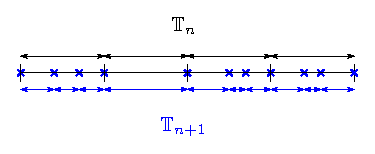
\includegraphics[width=0.5\textwidth]{MA3L13_3.eps}
		\label{MA3L13_3}
		\caption{Измельчение разбиения $\MTB_n$.}
		\label{fig:измельчение	}
	\end{figure}
	Пусть по утверждению $3$ мы выбрали $\VE > 0, \, \delta > 0$ и нашли $N \Rightarrow$ будем рассматривать при $n > N$ нижнюю сумму Дарбу:
	$$
		s(f_n, \MTB_n) = \sum\limits_{j \notin \MI}\inf\limits_{\Delta_j^n}f_n|\Delta_j^n| + \sum\limits_{j \in \MI}\inf\limits_{\Delta_j^n}f_n|\Delta_j^n|, \, \MI = \left\{j \colon \inf\limits_{\Delta_j^n}f_n \geq \VE\right\}
	$$
	следовательно, каждая из этих сумм легко оцениваются:
	$$
		\sum\limits_{j \notin \MI}\inf\limits_{\Delta_j^n}f_n|\Delta_j^n| < \VE \sum\limits_{j \notin \MI}|\Delta_j^n| \leq \VE\sum\limits_{j} |\Delta_j^n| = \VE (b-a)
	$$
	$$
		\sum\limits_{j \in \MI}\inf\limits_{\Delta_j^n}f_n|\Delta_j^n| \leq C \sum\limits_{j \in \MI}|\Delta_j^n| \leq C \delta
	$$
	Поскольку $\VE$ и $\delta$ были выбраны произвольно, то выбирая их маленькими, мы делаем и нижнюю сумму Дарбу маленькой. Пусть $\delta = \VE$ и выбираем $n$ так, чтобы $n > N$ и $\tfrac{1}{n} < \VE$, тогда:
	$$
		\forall \VE > 0, \, \exists \, N^\prime \colon \forall n > N^\prime, \, \ddint{a}{b}f_n(x)dx < \dfrac{1}{n} + s(f_n, \MTB_n) <  \VE ( 1 + (b-a) + C) = \VE C^\prime 
	$$
\end{proof}

\newpage

\subsection*{Теорема Арцела (второе доказательство)}
Есть множество доказательств этой теоремы (в том числе и ошибочных), попробуем доказать теорему без введения элементов теории меры (Люксембург). Будем обозначать нижний интеграл Дарбу следующим образом:
$$
	\lowint f(x)dx = \sup\limits_{\MTB}s(f,\MTB) = \lim\limits_{\lambda(\MTB) \to 0} s(f,\MTB), \, s(f, \MTB) = \sum\limits_{k = 1}^{N} \inf\limits_{\Delta_k}f{\cdot}|\Delta_k|
$$
Если $f$ - ограничена, то:
$$
	f(x) \in B(x) \Rightarrow\exists \, \displaystyle \lowint f(x)dx
$$ 
для ограниченной функции нижний и верхний интеграл Дарбу всегда существуют. Если функция интегрируема, то её нижний интеграл Дарбу совпадает с обычным интегралом Римана. Воспользуемся следующим:
$$
	f(x) \leq g(x) \Rightarrow \inf\limits_{\Delta_k} f(x) \leq f(x) \leq g(x) \leq \inf\limits_{\Delta_k} g(x)\Rightarrow s(f,\MTB) \leq s(g,\MTB) \Rightarrow \lowint f(x)dx \leq \lowint g(x) dx
$$
Таким образом, нижний интеграл Дарбу обладает свойством монотонности.
\begin{exrc}
	Доказать, что нижний интеграл Дарбу не обладает свойством линейности.
\end{exrc}
\begin{lemma}
	Пусть $f \geq 0$ и ограничена, тогда:
	$$
		\forall \VE> 0, \, \exists \, g_\VE \in C[a,b] \colon 0 \leq g_\VE(x) \leq f(x) \wedge \lowint\limits_{a}^{b} f(x)dx \leq \ddint{a}{b}g_\VE(x)dx + \VE
	$$
\end{lemma}
\begin{proof}
	По определению нижнего интеграла Дарбу (как точной верхней грани):
	$$
		\forall \VE > 0, \, \exists \, \MTB \colon \lowint\limits_{a}^{b}f(x)dx \leq s(f,\MTB) + \dfrac{\VE}{2}  
	$$
	Теперь хотелось бы понять, можно ли найти некоторую функцию $h(x)$ такую, что:
	$$
		s(f,\MTB) = \ddint{a}{b}h(x)dx
	$$
	Возьмем разбиение отрезка $\{\Delta_k\}$ и преобразуем отрезки в полуинтервалы так, чтобы:
	$$
		\forall k = \overline{1,N-1}, \, \Delta_k = [x_{k-1}, x_k] \Rightarrow \wte{\Delta}_k = [x_{k-1}, x_k), \, \Delta_N = \wte{\Delta}_N = [x_{N-1}, x_N]
	$$
	Это необходимо, чтобы на концах значения с использованием индикаторной функции не накладывались друг на друга. Таким образом, мы получим функцию $h(x)$:
	$$
		h(x) = \sum\limits_{k = 1}^N \inf\limits_{\Delta_k} f(x){\cdot}\MTI_{\wte{\Delta}_k}(x) = \sum\limits_{k = 1}^N c_k {\cdot}\MTI_{\wte{\Delta}_k}(x)
	$$
	Тогда по определению $h(x) \geq 0$, поскольку $f(x) \geq 0$ и $\forall x \in \wte{\Delta}_k$ будет верно, что $\inf\limits_{\Delta_k}f(x) \leq f(x)$, следовательно $0 \leq h(x) \leq f(x)$ и мы получаем:
	$$
		\lowint\limits_{a}^{b}f(x)dx \leq \ddint{a}{b}h(x)dx + \dfrac{\VE}{2}
	$$
	Полученная функция $h(x)$ плоха тем, что она разрывна, а мы хотим сделать её непрерывной, не сильно испортив интеграл от $h(x)$. Пусть $\delta > 0$, отступим от краев полуинтервалов на $\delta$: 
	$$
		\forall k = \overline{1,N-1},\, \wte{\Delta}_k = \left[x_{k-1}, x_k\right) \Rightarrow \wte{\Delta}_k = \left[x_{k-1}, x_{k-1}+\delta\right) \cup \left[x_{k-1} + \delta, x_k - \delta\right) \cup \left[x_k - \delta, x_k\right)
	$$
	$$
		\wte{\Delta}_N = \left[x_{N-1}, x_N\right] \Rightarrow \wte{\Delta}_N = \left[x_{N-1}, x_{N-1}+\delta \right) \cup\left[x_{N-1} + \delta, x_N - \delta\right) \cup \left[x_N - \delta, x_N\right]
	$$
	и построим ребра трапеции на промежутках $\left[x_{k-1}, x_{k-1}+\delta\right)$ и $\left[x_k - \delta, x_k\right)$, тогда получим функцию:
	\begin{figure}[H]
		\centering
		\includegraphics[width=0.5\textwidth]{MA3L13_5.eps}
		\label{MA3L13_5}
		\caption{Построение функции $h(x)$.}
		\label{fig:построение h(x)}
	\end{figure}
	$$
		g_{\delta}(x) = 
		\begin{cases}
			\dfrac{c_k}{\delta}(x - x_{k-1}), &x \in  \left[x_{k-1}, x_{k-1}+\delta\right) \\[4pt]
			c_k, & x \in \left[x_{k-1} + \delta, x_k - \delta\right)\\[4pt]
			\dfrac{c_k}{\delta}(x_k - x ), & x \in \left[x_k - \delta, x_k\right) \vee x \in [x_{N} - \delta, x_N]
		\end{cases}
	$$
	Очевидно, что $g_\delta(x) \in C[a,b]$ и $0 \leq g_\delta(x) \leq h(x)$. Пусть $\forall x \in [a,b], \, 0 \leq f(x) \leq C$, сравним интегралы (смотрим на разность площадей под графиками):
	$$
		\ddint{a}{b}h(x)dx - \ddint{a}{b}g_\delta(x)dx \leq c_1{\cdot}\delta{\cdot}\dfrac{1}{2}{\cdot}2 + c_2{\cdot}\delta{\cdot}\dfrac{1}{2}{\cdot}2 + \dotsc +  c_N{\cdot}\delta{\cdot}\dfrac{1}{2}{\cdot}2 \leq N\delta C
	$$
	Поскольку $N,C$ - фиксированы, то выберем $\delta$ так, чтобы $N\delta C < \tfrac{\VE}{2}$ и тогда функция $g_\delta$ - искомая.
\end{proof}
\begin{lemma}
	Пусть $0 \leq f_n \leq C$, $f_n \to 0$ и $\forall x, \, f_n(x) \geq f_{n+1}(x)$ (невозр. последовательность $\forall x$), тогда:
	$$
		\lowint\limits_{a}^{b}f_n(x)dx \to 0
	$$ 
\end{lemma}
\begin{proof}
	По лемме $1$:
	$$
		\forall n, \, \exists \, g_n \in C[a,b] \colon 0 \leq g_n \leq f_n, \,  \lowint\limits_{a}^{b}f_n(x)dx \leq \ddint{a}{b}g_n(x)dx + \dfrac{\VE}{2^n}
	$$
	Поскольку $\forall x, \, f_n(x) \to 0$, то из неравенства выше $\forall x, \, g_n(x) \to 0$, но вообще говоря ничего про монотонность сказать не можем. Перейдем к вспомогательным функциям $h_n(x)$:
	$$
		h_n(x) = \min\{g_1(x), g_2(x), \dotsc, g_n(x)\}
	$$
	Очевидно, что $h_n(x) \in C[a,b]$, в силу непрерывности функций $\{g_n(x)\}$ и функции $\min\{x_1, \dotsc, x_n\}$. Также ясно, что $h_n(x)$ не возрастает по $n$: $h_n(x) \geq h_{n+1}(x)$, более того $0 \leq h_n(x) \leq g_n(x) \Rightarrow \forall x, \, h_n(x) \to 0$ и по признаку Дини (будет дальше доказана в курсе) $h_n \uconv{} 0$. Тогда:
	$$
		\ddint{a}{b}h_n(x)dx \to 0
	$$
	Для доказательства леммы не хватает оценки разности интегралов по функциям $h_n(x)$ и $g_n(x)$, если они не отличаются сильно, то интеграл от $g_n(x)$ также будет стремится к нулю. Оценим разность:
	$$
		g_n(x) - h_n(x) = g_n(x) - \min\{g_1(x), \dotsc, g_n(x)\} \leq \sum\limits_{k = 1}^n \left(\max\{g_k(x),\dotsc,g_n(x)\} - g_k(x)\right)
	$$
	Каждое слагаемое справа - неотрицательное по построению суммы. Неравенство верно в силу того, что хотя бы одно слагаемое справа будет больше, чем слагаемое слева. Например, если $\min\{g_1(x), \dotsc, g_n(x)\} = g_m(x)$, то:
	$$
		 g_n(x) - \min\{g_1(x), \dotsc, g_n(x)\} = g_n(x) - g_m(x) \leq \max\{g_m(x), \dotsc, g_n(x)\} - g_m(x)
	$$
	Оценим интеграл разности:
	$$
		\ddint{a}{b} (g_n(x) - h_n(x))dx \leq \sum\limits_{k = 1}^n\left(\ddint{a}{b} \max\{g_k(x),\dotsc,g_n(x)\}dx - \ddint{a}{b}g_k(x)dx\right)
	$$
	Поскольку функции $f_n(x)$ - монотонные и в силу построения $g_n(x)$ будет верно: 
	$$
		\max\{g_k(x),\dotsc,g_n(x)\} \leq \max\{f_k(x),\dotsc,f_n(x)\} = f_k(x) \Rightarrow 
	$$
	$$
		\Rightarrow\ddint{a}{b} \max\{g_k(x),\dotsc,g_n(x)\}dx  = \lowint\limits_{a}^{b} \max\{g_k(x),\dotsc,g_n(x)\}dx \leq \lowint\limits_{a}^{b}f_k(x) dx
	$$
	где равенство верно в силу того, что интеграл Римана и Дарбу совпадают для $g_n(x)$, а неравенство верно в силу монотонности нижнего интеграла Дарбу. Тогда:
	$$
		\ddint{a}{b} \max\{g_k(x),\dotsc,g_n(x)\}dx - \ddint{a}{b}g_k(x)dx \leq \lowint\limits_{a}^{b}f_k(x) dx - \ddint{a}{b}g_k(x)dx \leq \dfrac{\VE}{2^k} \Rightarrow
	$$
	$$
		\Rightarrow \ddint{a}{b}\left(g_n(x) - h_n(x)\right)dx \leq \sum\limits_{k = 1}^n \left(\max\{g_k(x),\dotsc,g_n(x)\} - g_k(x)\right) \leq \sum\limits_{k = 1}^{n}\dfrac{\VE}{2^k} \leq \VE
	$$
	Таким образом, мы получаем:
	$$
		\forall \VE > 0, \, \lowint\limits_{a}^{b}f_n(x)dx \leq \ddint{a}{b}g_n(x)dx + \dfrac{\VE}{2^n} \leq \ddint{a}{b}g_n(x)dx + \VE \leq  \ddint{a}{b}h_n(x)dx + 2\VE
	$$
	Поскольку $\VE$ - произвольный, интеграл от $h_n(x)$ стремится к нулю, то:
	$$
		\ddint{a}{b}h_n(x)dx \to 0 \Rightarrow \lowint\limits_{a}^{b}f_n(x)dx \to 0
	$$
\end{proof}

\begin{theorem}(\textbf{Арцела})
	Если $f_n, f$ - интегрируемы на $[a,b]$ по Риману, последовательность - ограничена: $\forall n, x, \, |f_n(x)| \leq C$ (равномерно ограничены) и $f_n(x) \to f(x)$ поточечно, то:
	$$
		\lim\limits_{n \to \infty} \ddint{a}{b}f_n(x) dx = \ddint{a}{b}f(x)dx
	$$
\end{theorem}
\begin{proof}
	Достаточно доказать только в следующем частном случае:
	$$
		C \geq f_n \geq 0, \, f_n \to 0 \Rightarrow \ddint{a}{b}f_n(x)dx \to 0
	$$
	Для понимания этого факта, рассмотрим следующую разность:
	$$
		\left|\ddint{a}{b}f_n(x)dx - \ddint{a}{b}f(x)dx\right| \leq \ddint{a}{b}\left|f_n(x) - f(x)\right|dx \to 0 
	$$
	где верно следующее: $\forall n, \, |f_n(x) - f(x) | \geq 0 \wedge \lim\limits_{n \to \infty}|f_n(x) - f(x)| = 0$. Таким образом, это эквивалентно нашему частному случаю. Введем вспомогательные функции:
	$$
		\forall n, \, M_n(x) = \sup\limits_{k \geq n}f_k(x)
	$$
	Тогда для этих функций будет справедливо: $0 \leq M_n(x) \leq C$ и $M_n(x) \geq M_{n + 1}(x)$ просто по определению, поскольку $\lim\limits_{n \to \infty}f_n(x) = 0$, то $\lim\limits_{n \to \infty} M_n(x) = 0$. Однако, про интегрируемость $M_n(x)$ мы уже ничего сказать не можем. Также очевидно, что 
	$$
		\forall n, \, 0 \leq f_n(x) \leq M_n(x)
	$$
	Поскольку нижний интеграл Дарбу обладает свойством монотонности, то в силу интегрируемости $f_n(x)$ по Риману будет верно:
	$$
		0 \leq \ddint{a}{b}f_n(x)dx = \lowint\limits_{a}^{b}f_n(x)dx \leq \lowint\limits_{a}^{b}M_n(x)dx
	$$
	По лемме $2$, второй интеграл будет стремиться к нулю.
\end{proof}


\newpage

\subsection*{Перестановочность равномерной сходимости и дифференцирования}
Заметим, что не существует  результата, который утверждал что если последовательность дифференцируемых функций сходится равномерно, то можно говорить, что её предел будет дифференцируемой функцией. Легко придумать последовательность функций:
$$
	f_n(x) = \dfrac{\sin{(n^2 x)}}{n} \uconv{} 0, \, f^\prime_n(x) = n\cos{(n^2x)} \Rightarrow \nexists \lim\limits_{n \to \infty}f_n^\prime(x)
$$
где последовательность их производных $f_n^\prime$ не будут сходиться (даже поточечно). Поэтому результаты с производными обычно формулируются задом наперед: если всё хорошо с производными, а с функциями не слишком плохо, то с функциями всё хорошо.
\begin{rem}
	Заметим, что если последовательность производных $f_n^\prime$ равномерно сходится, то из этого, вообще говоря, не следует, что $f_n$ куда-либо тоже сходятся. Например, можно взять последовательность констант и тогда:
	$$
		f_n^\prime(x) \uconv{} 0 \nRightarrow \exists \, g \colon f_n \to g
	$$
\end{rem}

\begin{theorem}
	Пусть функции $f_n$ - дифференцируемы на $(a,b)$, $f_n^\prime \uconv{(a,b)} g$ и $\exists \, x_0 \in (a,b) \colon \exists \, \lim\limits_{n \to \infty} f_n(x_0)$. Тогда  эти функции сходятся равномерно: $f_n \uconv{(a,b)} f$
	и $f$ - дифференцируема на $(a,b)$, причем $f^\prime = g$.
\end{theorem}
\begin{proof}
	Покажем сначала, что последовательность $f_n$ сходится. Воспользуемся критерием Коши:
	$$
		\forall n,m, \, f_n(x) - f_m(x) = (f_n(x) - f_m(x)) - (f_n(x_0) - f_m(x_0)) + (f_n(x_0) - f_m(x_0))
	$$
	Таким образом, первые два слагаемых образуют приращение, тогда как для последнего слагаемого, в силу сходимости в точке $x_0$, критерий выполняется. Воспользуемся теоремой Лагранжа:
	$$
		 \exists \, c \in (x_0, x) \vee c \in (x, x_0), \, f_n(x) - f_m(x) - (f_n(x_0) - f_m(x_0)) = \left(f_n^\prime(c) - f_m^\prime(c)\right)(x - x_0)
	$$
	Тогда получим следующую оценку:
	$$
		|f_n(x) - f_m(x)| \leq |x - x_0|{\cdot}|f_n^\prime(c) - f_m^\prime(c)| + |f_n(x_0) - f_m(x_0)| 
	$$
	Переходя к точной верхней грани:
	$$
		\sup\limits_{(a,b)}|f_n(x) - f_m(x)| \leq (b - a){\cdot}\sup\limits_{(a,b)}|f_n^\prime(x) - f_m^\prime(x)|+ |f_n(x_0) - f_m(x_0)| 
	$$
	Поскольку $f_n^\prime$ сходится равномерно, то для неё выполняется критерий Коши. Поскольку $f_n(x_0)$ это числовая последовательность, которая сходится, то для неё он также выполняется. Тогда:
	$$
		(b - a){\cdot}\sup\limits_{(a,b)}|f_n^\prime(x) - f_m^\prime(x)|+ |f_n(x_0) - f_m(x_0)|  \xrightarrow[n,m \to \infty]{} 0 \Rightarrow \sup\limits_{(a,b)}|f_n(x) - f_m(x)| \xrightarrow[n,m \to \infty]{}  0
	$$
	Следовательно, для $f_n$ выполняется условие Коши равномерной сходимости $\Rightarrow f_n \uconv{(a,b)} f$. 
	
	Теперь хотелось бы понять, что $f$ - дифференцируемая и её производная в точности равна $g$. Пусть:
	$$
		h_n(x) = \dfrac{f_n(x) - f_n(x_0)}{x -x_0}, \, h(x) = \dfrac{f(x) - f(x_0)}{x - x_0} \Rightarrow \lim\limits_{x \to x_0} h_n(x) = f_n^\prime(x_0)
	$$ 
	то есть, при каждом $n$ функция $h_n$ имеет предел при $x \to x_0$. Мы хотим доказать, что: 
	$$
		\exists \, \lim\limits_{x \to x_0}h(x) \colon 	\lim\limits_{x \to x_0}h(x) = \lim\limits_{n \to \infty}f^\prime_n(x_0)
	$$
	Чтобы воспользоваться первой теоремой о перестановке пределов, надо проверить, что $h_n$ равномерно сходится к $h$. Очевидно, что $\forall x \neq x_0, \, h_n(x) \to h(x)$ поточечно (только что доказали). Проверим критерий Коши и вновь воспользуемся теоремой Лагранжа:
	$$
		h_n(x) - h_m(x) = \dfrac{(f_n(x) - f_m(x)) - (f_n(x_0) - f_m(x_0))}{x - x_0} = \dfrac{(f_n^\prime(t) - f_m^\prime(t))(x - x_0)}{x - x_0} = f_n^\prime(t) - f_m^\prime(t)
	$$
	где $t$ лежит между $x$ и $x_0$. Аналогично шагам ранее, возьмем точную верхнюю грань:
	$$
		\sup\limits_{(a,b)}|h_n(x) - h_m(x)| \leq \sup\limits_{(a,b)} | f_n^\prime(x) - f_m^\prime(x)|  \xrightarrow[n,m \to \infty]{}  0 \Rightarrow h_n(x) \uconv{(A,b)}h(x)
	$$
	Следовательно, по теореме о перестановке пределов функция $f$ будет дифференцируемой, причем:
	$$
		g(x_0) = \lim\limits_{n \to \infty} f_n^\prime(x_0) = \lim\limits_{n \to \infty}  \left(\lim\limits_{x \to x_0} h_n(x)\right) = \lim\limits_{x \to x_0}\bigg(\lim\limits_{n \to \infty}h_n(x)\bigg) = \lim\limits_{x \to x_0} h(x) = f^\prime(x_0)
	$$
	где последнее равенство верно просто по определению производной.
\end{proof}
\begin{rem}
	Заметим, что предположение о конечности интервала здесь важно. Например, если взять следующие функции:
	$$
		f_n(x) = \dfrac{x}{n}, \, x \in \MR \Rightarrow f_n(0) = 0 \to 0,\, f^\prime(x) = \dfrac{1}{n} \uconv{\MR} 0
	$$
	Но при этом сама функция $f_n(x) \not\uconv{\MR} 0$.
\end{rem}

\newpage
\section*{Функциональные ряды}
Очень часто последовательность приходит как последовательность частичных сумм. Поэтому рассмотрим ряды, каждым членом которого есть некоторая функция $f_n(x)$.
\begin{defn}
	Ряд $\displaystyle \sum\limits_{n = 1}^{\infty}f_n(x)$ \uwave{сходится поточечно на} $X \Leftrightarrow \forall x \in X, \, \displaystyle \sum\limits_{n = 1}^{\infty}f_n(x)$ - сходится.
\end{defn}
\begin{defn}
	Ряд $\displaystyle \sum\limits_{n = 1}^{\infty}f_n(x)$ \uwave{сходится равномерно на} $X \Leftrightarrow $ последовательность $S_N(x) = \displaystyle\sum\limits_{n = 1}^N f_n(x)$ частичных сумм этого ряда  сходится равномерно на $X$.
\end{defn}
Тем самым, ничего нового не возникает: исследование равномерной сходимости ряда это исследование равномерной сходимости его частичных сумм. 
\begin{rem}
	Из определения сразу следует, что если ряд сходится равномерно, то он должен быть сходящимся $\Rightarrow$ всегда предполагаем ряд сходящимся.
\end{rem}
Пусть ряд $\displaystyle \sum\limits_{n = 1}^{\infty}f_n(x)$ сходится поточечно. Что означает его равномерная сходимость? Рассмотрим хвост этой суммы:
$$
	\sum\limits_{n = N+1}^{\infty} f_n(x) = S(x) - S_N(x) \Rightarrow \sup\limits_X \left|\sum\limits_{n = N+1}^{\infty} f_n(x) \right|= \sup\limits_X \left|S(x) - S_N(x)\right| \xrightarrow[N \to \infty]{} 0
$$
то есть равномерная сходимость ряда это в точности равномерная сходимость к нулю его хвостов. Сразу же из определения следует утверждение, которое часто работает на практике.
\begin{prop}(\textbf{необходимое условие равномерной сходимости ряда})
	Если ряд $\displaystyle \sum\limits_{n = 1}^{\infty}f_n(x)$ сходится равномерно на $X$, то его слагаемые равномерно стремятся к нулю: $f_n \uconv{X}0$.
\end{prop}
\begin{proof}
	$$
		f_n(x) = S_n(x) - S_{n-1}(x), \, S_n(x) \uconv{X} S(x), \, S_{n-1}(x) \uconv{X} S(x) \Rightarrow f_n(x) \uconv{X} S(x) - S(x) = 0
	$$
\end{proof}

\begin{theorem}(\textbf{критерий Коши равномерной сходимости ряда})
	Ряд $\displaystyle \sum\limits_{n = 1}^{\infty}f_n(x)$ сходится равномерно на $X$ тогда и только тогда, когда:
	$$
		\forall \VE > 0, \, \exists \, N \colon \forall n,m > N, \, \sup\limits_{X}\left| \sum\limits_{k = m}^{n} f_k(x)\right| < \VE
	$$
\end{theorem}
\begin{proof}
	Этот критерий есть буквально переписанная теорема для последовательности частичных сумм, поскольку:
	$$
		\sup\limits_{X}\left| \sum\limits_{k = m}^{n} f_k(x)\right| = \sup\limits_{X}\left| S_n(x) - S_m(x) \right|
	$$
\end{proof}
Основной и самый популярный метод проверки рядов на наличие равномерной сходимости это признак Вейерштрасса.
\begin{theorem}(\textbf{признак Вейерштрасса})
	Пусть $f_n \colon X \to \MR$ и $\exists \, a_n \geq 0 \colon \forall x \in X, \, |f_n(x)| \leq a_n$, тогда из сходимости ряда $\displaystyle \sum\limits_{n = 1}^{\infty}a_n$ следует равномерная сходимость ряда $\displaystyle \sum\limits_{n = 1}^{\infty}f_n(x)$.
\end{theorem}
\begin{proof}
	Проверим критерий Коши:
	$$
		\forall x \in X, \, \left| \sum\limits_{k = m}^{n} f_k(x)\right| \leq \sum\limits_{k = m}^n a_k \Rightarrow \sup\limits_{X}\left| \sum\limits_{k = m}^{n} f_k(x)\right| \leq \sum\limits_{k = m}^n a_k
	$$
	Поскольку для ряда $\displaystyle \sum\limits_{n = 1}^{\infty}a_n$ критерий Коши выполняется и оценка сверху не зависит от $x$, то критерий Коши для функционального ряда сразу выполняется.
\end{proof}
\begin{rem}
	Заметим, что признак Вейерштрасса используется не только для рядов, но и для последовательностей, поскольку:
	$$
		f_n = f_1 + f_2 - f_1 + f_3 - f_2 + \dotsc + f_n - f_{n-1}
	$$
	В этом случае признак Вейерштрасса означает, что для равномерной сходимости последовательности достаточно иметь оценку разности соседей $f_n$:
	$$
		|f_n - f_{n-1}| \leq a_n 
	$$
	Следовательно, если ряд из $a_n$ сойдется, то из этого будет следовать, что $f_n$ сойдутся равномерно:
	$$
		\sum\limits_{n = 1}^{\infty}a_n < \infty \Rightarrow f_n \uconv{} f
	$$
\end{rem}
Также вспомним теорему, уже доказанную для последовательностей.
\begin{theorem}
	Пусть $(X,\rho)$ - метрическое пространство, $a$ - предельная точка, $f_n \colon X\setminus \{a\} \to \MR(\MC)$ и $\forall n, \, \exists \, \lim\limits_{x \to a} f_n(x) = b_n$. Если ряд $\displaystyle \sum\limits_{n = 1}^{\infty}f_n(x)$ сходится равномерно на $X \setminus \{a\}$ и его сумма равна $S(x)$, то $\exists \, \lim\limits_{x \to a} S(x)\colon \sum\limits_{n = 1}^{\infty}b_n = \lim\limits_{x \to a} S(x) < \infty$
	Или если написать подробнее:
	$$
		\sum\limits_{n = 1}^{\infty}\lim\limits_{x \to a}f_n(x) = \lim\limits_{x \to a} \sum\limits_{n =1}^{\infty}f_n(x) < \infty
	$$
\end{theorem}
\begin{proof}
	Поскольку $S_N(x) \uconv{} S(x)$, при этом если возьмем предел при $x \to a$, то:
	$$
		\lim\limits_{x \to a}S_N(x) = \sum\limits_{n = 1}^{N} b_n
	$$
	Далее воспользуемся теоремой о перестановке пределов:
	$$
		\sum\limits_{n = 1}^{\infty}b_n = \lim\limits_{N \to \infty}\sum\limits_{n = 1}^{N} b_n = \lim\limits_{N \to \infty}\left(\lim\limits_{x \to a}S_N(x)\right) = \lim\limits_{x \to a}\left(\lim\limits_{N \to \infty}S_N(x)\right) = \lim\limits_{x \to a} S(x) = \lim\limits_{x \to a}\sum\limits_{n =1}^{\infty}f_n(x)
	$$
\end{proof}

\newpage
\subsection*{Переформулировки некоторых теорем для рядов}
\begin{theorem}(\textbf{о перестановке ряда и интеграла})
	Пусть функции $f_n(x)$ - интегрируемы по Риману на $[a,b]$ и ряд $\ddsum{n = 1}{\infty}f_n$ сходится равномерно на $[a,b]$ к своей сумме $S(x)$. Тогда $S(x)$ - интегрируема по Риману и верно:
	$$
		\ddint{a}{b}S(x)dx = \ddsum{n = 1}{\infty}\ddint{a}{b}f_n(x)dx
	$$
\end{theorem}
\begin{proof}
	Распишем частичную сумму, как последовательность и применим теорему о перестановке пределов:
	$$
		S_N(x) = \ddsum{n = 1}{N}f_n(x) \Rightarrow S_N(x) \uconv{[a,b]} S(x) \Rightarrow \ddint{a}{b}S(x)dx = \lim\limits_{N \to \infty}\ddint{a}{b}S_N(x)dx = \lim\limits_{N \to \infty}\ddsum{n = 1}{N}\ddint{a}{b}f_n(x)dx
	$$
\end{proof}

\begin{theorem}(\textbf{о дифференцируемости суммы ряда})
	Пусть функции $f_n(x)$ дифференцируемы на конечном интервале $(a,b)$, $\exists \,  x_0 \colon$ ряд $\ddsum{n = 1}{\infty}f_n(x_0)$ сходится и ряд $\ddsum{n = 1}{\infty}f_n^\prime(x)$ сходится на $(a,b)$ равномерно. Тогда $\ddsum{n  = 1}{\infty}f_n(x)$ сходится равномерно на $(a,b)$, его сумма $S(x)$ - дифференцируема на $(a,b)$ и верно:
	$$
		S^\prime(x) = \ddsum{n = 1}{\infty}f_n^\prime(x)
	$$ 
\end{theorem}
\begin{proof}
	Распишем частичную сумму, как последовательность:
	$$
		S_N(x) = \ddsum{n = 1}{N}f_n(x) \Rightarrow S_N^\prime(x) = \ddsum{n = 1}{N}f_n^\prime(x) \uconv{(a,b)} g(x), \, \exists \, \lim\limits_{N \to \infty}S_N(x_0) = \ddsum{n = 1}{\infty}f_n(x_0)
	$$
	Тогда по теореме о перестановке дифференцируемости и предела:
	$$
		S_N(x) \uconv{(a,b)} S(x), \, S^\prime(x) = g(x) = \lim\limits_{N\to \infty}S_N^\prime(x) = \ddsum{n = 1}{\infty}f_n^\prime(x)
	$$
\end{proof}

\end{document}